\documentclass[border=3pt,tikz]{standalone}
% Gemeinsame Praeambel aller Abbildungen — Palette und Styles identisch zum
% GermEval-2026-Paper (Nuernberg NLP), damit die Bilder dort wiederverwendbar
% sind, ohne neu gezeichnet zu werden.
\usepackage{xcolor}
\usepackage{ifthen}
\usepackage{tikz}
\usetikzlibrary{shapes,arrows.meta,positioning,fit,backgrounds,calc,decorations.pathreplacing}

\definecolor{clrPrompt}{HTML}{B0CA97} % green  — Prompting (baseline)
\definecolor{clrSFT}{HTML}{E8A087}    % salmon — SFT (generative)
\definecolor{clrCls}{HTML}{88C4C8}    % teal   — ClsHead / FT (discriminative)
\definecolor{clrEns}{HTML}{D1BC8A}    % gold   — ensemble / majority vote
\definecolor{clrPCS}{HTML}{B7A0C9}    % purple — minority-class scope
\definecolor{clrBase}{HTML}{9AA0A6}   % grey   — untrained/frozen base

\tikzset{
  sysbox/.style={rectangle, rounded corners=3pt, line width=0.9pt,
    minimum width=2.7cm, minimum height=0.82cm, align=center,
    inner ysep=2pt, inner xsep=4pt, font=\fontsize{7.5}{9}\selectfont\bfseries},
  voterchip/.style={rectangle, rounded corners=1.5pt, line width=0.55pt,
    minimum width=0.78cm, minimum height=0.36cm, align=center,
    inner sep=1pt, font=\fontsize{5.4}{6.4}\selectfont},
  major/.style={rectangle, rounded corners=3pt, line width=0.9pt,
    align=center, font=\footnotesize\bfseries, inner ysep=4pt, inner xsep=10pt},
  io/.style={rectangle, rounded corners=2pt, line width=0.55pt, align=center,
    minimum width=1.35cm, minimum height=0.72cm, fill=black!3, draw=black!35,
    font=\fontsize{7.2}{8.6}\selectfont},
  bb/.style={rectangle, rounded corners=3pt, line width=0.8pt, align=center,
    minimum width=2.35cm, minimum height=0.86cm,
    font=\fontsize{7.4}{8.8}\selectfont},
  lab/.style={rectangle, rounded corners=1.2pt, line width=0.45pt,
    minimum height=0.30cm, align=center, inner sep=1.5pt,
    font=\fontsize{5.6}{6.8}\selectfont},
  edge/.style={-{Stealth[length=4pt]}, line width=0.6pt, black!50},
  bus/.style={line width=0.6pt, black!50},
  note/.style={font=\fontsize{6.4}{7.8}\selectfont\itshape, text=black!55,
    align=center},
  hdr/.style={font=\fontsize{6.5}{8}\selectfont\bfseries, text=black!55},
}

\begin{document}
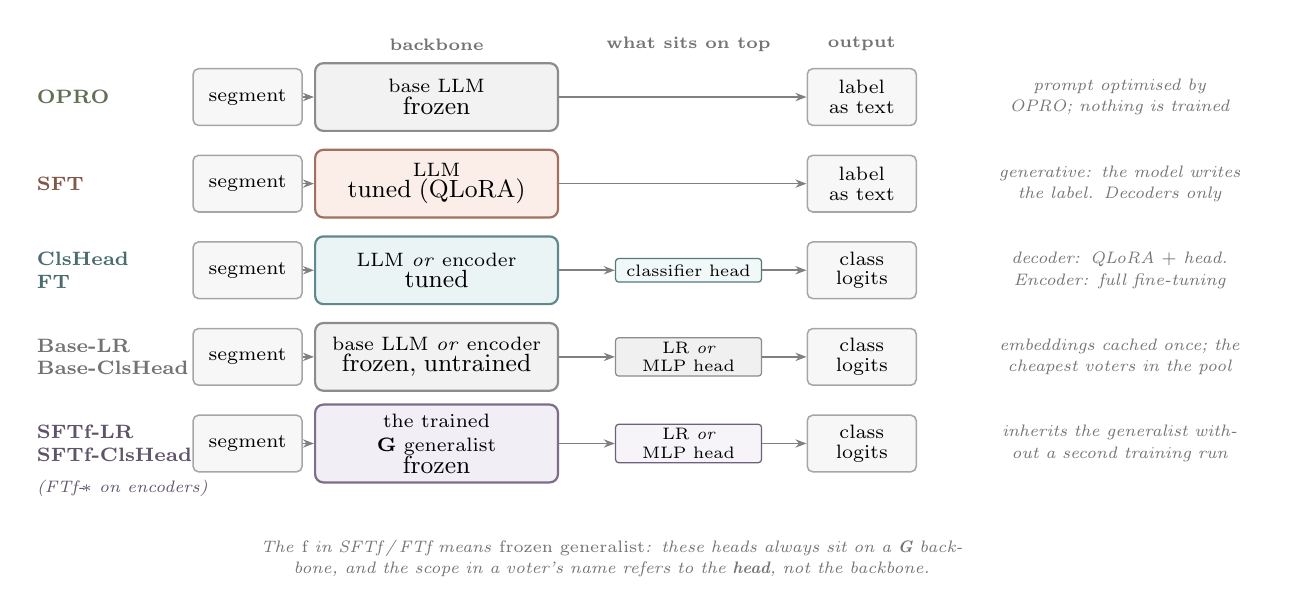
\begin{tikzpicture}[
  rowlab/.style={font=\fontsize{7}{8.2}\selectfont\bfseries, anchor=west, align=left},
  small/.style={font=\fontsize{5.9}{7.2}\selectfont\mdseries},
  % feste Spaltenbreiten: sonst wachsen die Boxen mit ihrem Text und
  % schieben sich ueber die Nachbarspalte.
  bb/.append style={text width=2.85cm, minimum width=3.05cm},
  io/.append style={text width=1.15cm, minimum width=1.35cm},
  lab/.append style={text width=1.75cm, minimum width=1.95cm},
]

\def\xin{-5.95}
\def\xbb{-3.55}
\def\xhd{-0.35}
\def\xout{1.85}
\def\xnote{3.25}

% ── column headers ─────────────────────────────────────────────────────────
\node[hdr] at (\xbb, 2.92) {\textsc{backbone}};
\node[hdr] at (\xhd, 2.92) {\textsc{what sits on top}};
\node[hdr] at (\xout, 2.92) {\textsc{output}};

% ── row 1: prompting ───────────────────────────────────────────────────────
\node[rowlab, text=clrPrompt!55!black] at (-8.75, 2.25) {OPRO};
\node[io] (i1) at (\xin, 2.25) {segment};
\node[bb, draw=black!45, fill=black!5] (b1) at (\xbb, 2.25)
  {base LLM\\[-1pt]{\small frozen}};
\node[io] (o1) at (\xout, 2.25) {label\\[-1.5pt]as text};
\draw[edge] (i1) -- (b1);
\draw[edge] (b1) -- (o1);
\node[note, anchor=west, text width=3.5cm] at (\xnote, 2.25)
  {prompt optimised by OPRO; nothing is trained};

% ── row 2: SFT ─────────────────────────────────────────────────────────────
\node[rowlab, text=clrSFT!55!black] at (-8.75, 1.15) {SFT};
\node[io] (i2) at (\xin, 1.15) {segment};
\node[bb, draw=clrSFT!70!black, fill=clrSFT!18] (b2) at (\xbb, 1.15)
  {LLM\\[-1pt]{\small tuned (QLoRA)}};
\node[io] (o2) at (\xout, 1.15) {label\\[-1.5pt]as text};
\draw[edge] (i2) -- (b2);
\draw[edge] (b2) -- (o2);
\node[note, anchor=west, text width=3.5cm] at (\xnote, 1.15)
  {generative: the model writes the label. Decoders only};

% ── row 3: ClsHead / FT ────────────────────────────────────────────────────
\node[rowlab, text=clrCls!55!black] at (-8.75, 0.05) {ClsHead\\FT};
\node[io] (i3) at (\xin, 0.05) {segment};
\node[bb, draw=clrCls!70!black, fill=clrCls!18] (b3) at (\xbb, 0.05)
  {LLM \emph{or} encoder\\[-1pt]{\small tuned}};
\node[lab, draw=clrCls!62!black, fill=clrCls!12, minimum width=1.5cm] (h3)
  at (\xhd, 0.05) {classifier head};
\node[io] (o3) at (\xout, 0.05) {class\\[-1.5pt]logits};
\draw[edge] (i3) -- (b3);
\draw[edge] (b3) -- (h3);
\draw[edge] (h3) -- (o3);
\node[note, anchor=west, text width=3.5cm] at (\xnote, 0.05)
  {decoder: QLoRA $+$ head. Encoder: full fine-tuning};

% ── row 4: Base-LR / Base-ClsHead ──────────────────────────────────────────
\node[rowlab, text=black!55] at (-8.75, -1.05) {Base-LR\\Base-ClsHead};
\node[io] (i4) at (\xin, -1.05) {segment};
\node[bb, draw=black!45, fill=black!5] (b4) at (\xbb, -1.05)
  {base LLM \emph{or} encoder\\[-1pt]{\small frozen, untrained}};
\node[lab, draw=black!45, fill=black!6, minimum width=1.5cm] (h4)
  at (\xhd, -1.05) {LR \emph{or} MLP head};
\node[io] (o4) at (\xout, -1.05) {class\\[-1.5pt]logits};
\draw[edge] (i4) -- (b4);
\draw[edge] (b4) -- (h4);
\draw[edge] (h4) -- (o4);
\node[note, anchor=west, text width=3.5cm] at (\xnote, -1.05)
  {embeddings cached once; the cheapest voters in the pool};

% ── row 5: SFTf / FTf ──────────────────────────────────────────────────────
\node[rowlab, text=clrPCS!52!black] at (-8.75, -2.15) {SFTf-LR\\SFTf-ClsHead};
\node[rowlab, text=clrPCS!52!black, font=\fontsize{6.2}{7.4}\selectfont\itshape]
  at (-8.75, -2.72) {(FTf-\!$\ast$ on encoders)};
\node[io] (i5) at (\xin, -2.15) {segment};
\node[bb, draw=clrPCS!68!black, fill=clrPCS!18] (b5) at (\xbb, -2.15)
  {the trained \textbf{G} generalist\\[-1pt]{\small frozen}};
\node[lab, draw=clrPCS!60!black, fill=clrPCS!12, minimum width=1.5cm] (h5)
  at (\xhd, -2.15) {LR \emph{or} MLP head};
\node[io] (o5) at (\xout, -2.15) {class\\[-1.5pt]logits};
\draw[edge] (i5) -- (b5);
\draw[edge] (b5) -- (h5);
\draw[edge] (h5) -- (o5);
\node[note, anchor=west, text width=3.5cm] at (\xnote, -2.15)
  {inherits the generalist without a second training run};

% ── footnote on naming ─────────────────────────────────────────────────────
\node[note, anchor=north west, text width=14.6cm] at (-8.75, -3.25)
  {The \emph{f} in SFTf\,/\,FTf means \emph{frozen generalist}: these heads always
   sit on a \textbf{G} backbone, and the scope in a voter's name refers to the
   \textbf{head}, not the backbone.};

\end{tikzpicture}
\end{document}
